\documentclass{article}
\usepackage{graphicx}
\usepackage{geometry}
\usepackage[MeX]{polski}
\usepackage[polish]{babel}
\usepackage{float}
\usepackage{fancyhdr}
\newcommand{\q}[1]{„#1“}
\usepackage{caption}
\usepackage{xcolor}
\usepackage[most]{tcolorbox}
\usepackage[scaled=0.85]{FiraMono} 

\usepackage[T1]{fontenc}
\usepackage{listings}
\usepackage[utf8]{inputenc}
\setlength{\parindent}{0pt} 

\newtcblisting{mylisting}{
arc=2mm,
top=0mm,
bottom=0mm,
left=3mm,
right=0mm,
boxrule=1pt,
colback=black!85,
listing only,
listing options={
basicstyle=\ttfamily\color{white},
showstringspaces=false,
language=Python,
keywordstyle=\color{myorange},
stringstyle=\color{mygreen},
commentstyle=\color{mygray}
xleftmargin=.2\textwidth, xrightmargin=.2\textwidth
}
}

\renewcommand{\labelenumii}{\arabic{enumi}.\arabic{enumii}}
\renewcommand{\labelenumiii}{\arabic{enumi}.\arabic{enumii}.\arabic{enumiii}}
\renewcommand{\labelenumiv}{\arabic{enumi}.\arabic{enumii}.\arabic{enumiii}.\arabic{enumiv}}

\definecolor{mygreen}{RGB}{26, 171, 26}
\definecolor{myorange}{RGB}{230,110,20}
\definecolor{mygray}{RGB}{100,100,100}


\tcbuselibrary{listings}

\begin{document}
\begin{center}\vspace{-1cm}
    \textbf{ \Huge Wykrywanie naczyń dna \\siatkówki oka}\\
    \LARGE Informatyka w medycynie\\
    \Large Zuzanna Cienka  \\
    \large nr albumu 148201\\
    \large \today \\~\\
\end{center}

\begin{enumerate}

    \item Zastosowany język programowania oraz dodatkowe biblioteki.
          \begin{itemize}
              \item Python
              \item OpenCV
              \item Numpy
              \item Matplotlib
              \item Scikit image
          \end{itemize}
    \item Opis zastosowanych metod:
          \begin{enumerate}
              \item Przetwarzanie obrazów
                    \begin{enumerate}
                        \item Wstępne przetwarzanie obrazów\\
                              Podczas wstępnego przetwarzania wyodrębniany jest kanał zielony,
                              następnie obraz jest rozmywany, a potem usuwany jest szum i przeprowadzane jest
                              wyostrzanie obrazu. Następnie wykonywana jest normalizacja histogramu i
                              wzmocnienie naczyń krwionośnych filtrem Franghiego.
                              \begin{figure}[h]
                                  \centering
                                  \begin{minipage}{0.47\textwidth}
                                      \centering
                                      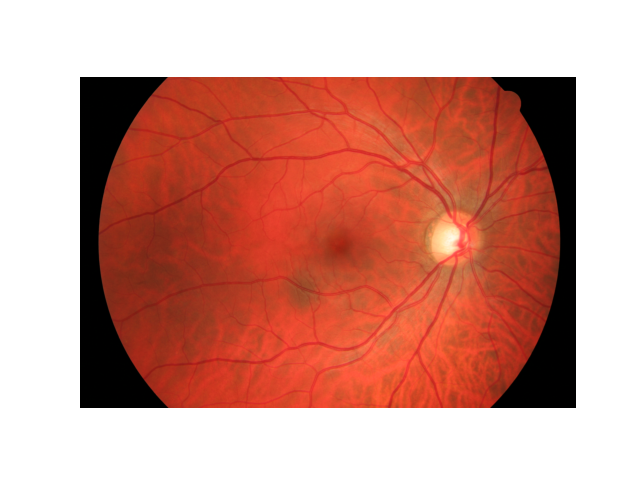
\includegraphics[width=\linewidth]{../res/sample-original-image.png}
                                  \end{minipage}
                                  \begin{minipage}{0.47\textwidth}
                                      \centering
                                      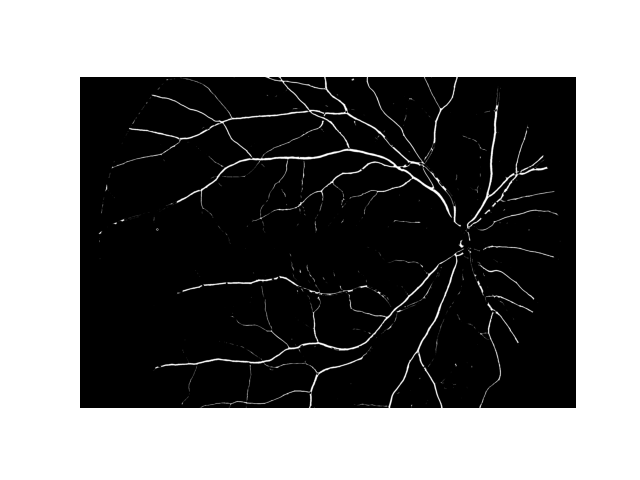
\includegraphics[width=\linewidth]{../res/sample-preprocessed-image.png}
                                  \end{minipage}
                                  \caption{Obraz przed i po przetworzeniu}
                              \end{figure}
                              \newpage
                        \item Przetworzone obrazy siatkówki oka\\
                              \begin{figure}[h]
                                  \centering
                                  \begin{minipage}{0.73\textwidth}
                                      \centering
                                      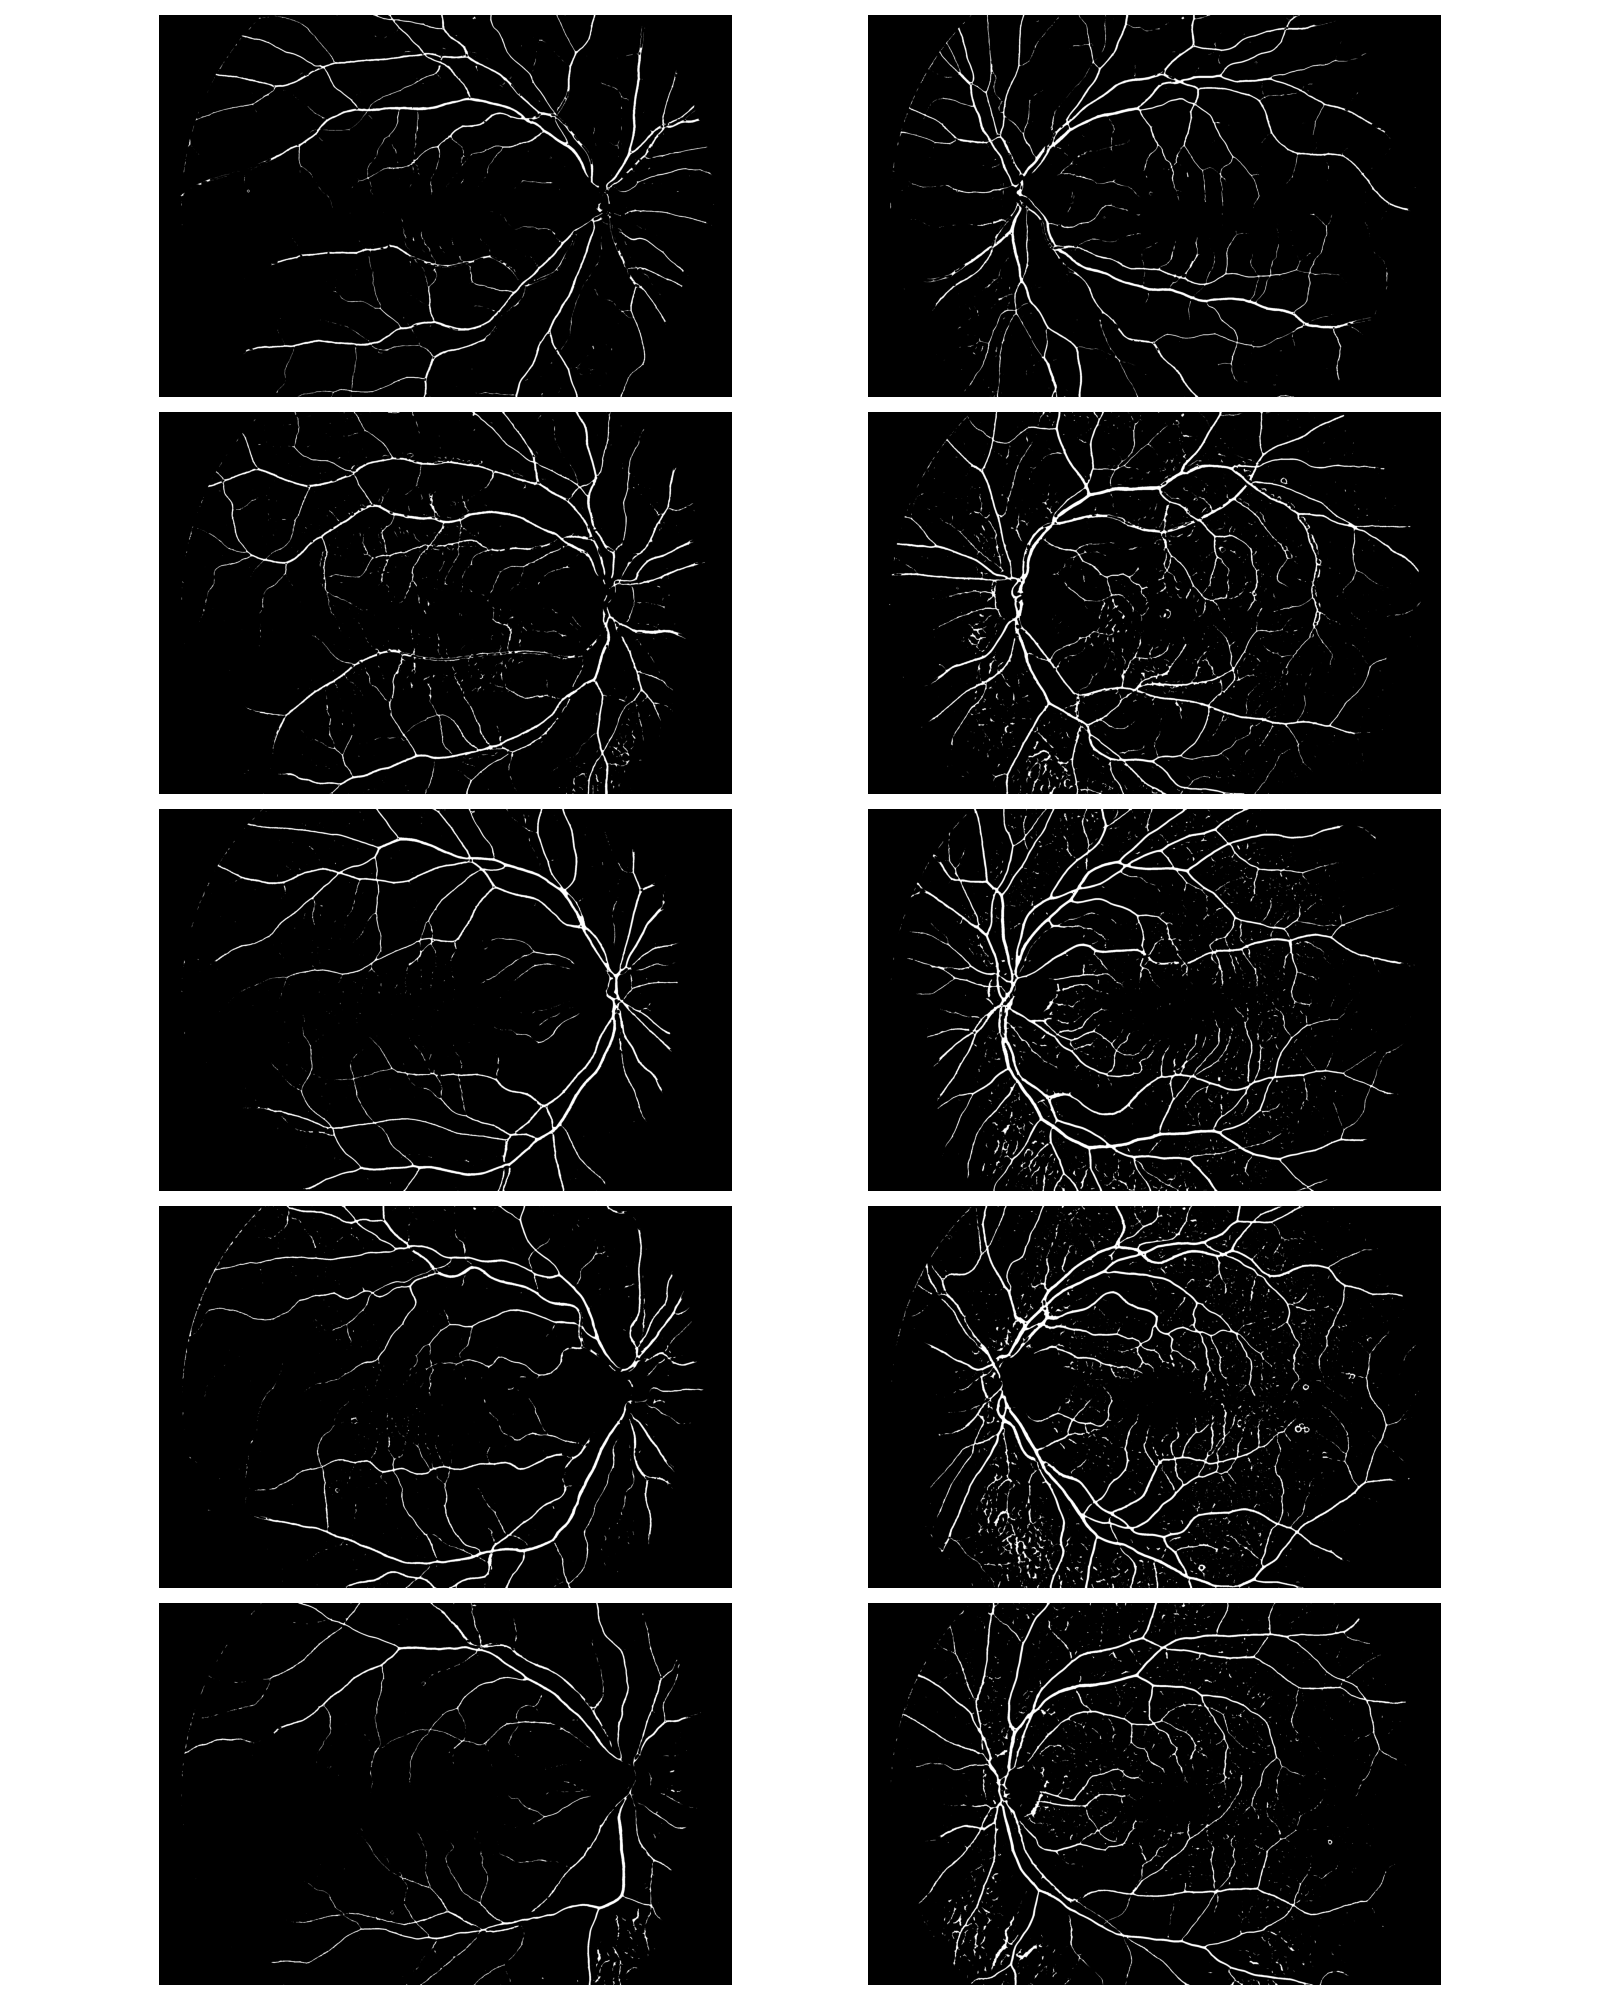
\includegraphics[width=0.73\linewidth]{../res/preprocessed-images.png}
                                  \end{minipage}
                              \end{figure}
                              \newpage
                        \item Zwizualizowane naczynia na oryginalnych zdjęciach\\
                              \begin{figure}[h]
                                  \centering
                                  \begin{minipage}{0.73\textwidth}
                                      \centering
                                      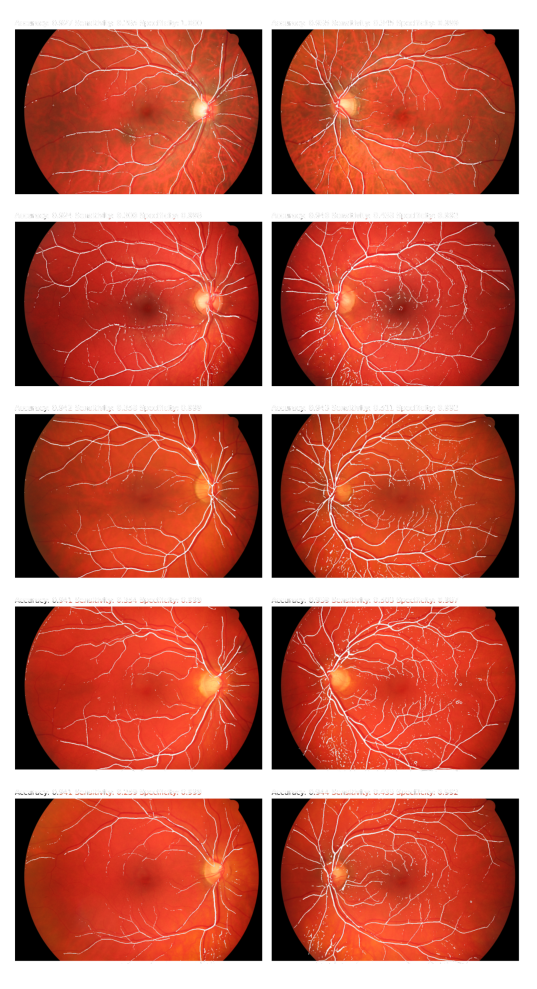
\includegraphics[width=0.73\linewidth]{../res/original-images-vessels-visualizedpng.png}
                                  \end{minipage}
                              \end{figure}
                    \end{enumerate}


                    \newpage
              \item Uczenie maszynowe
                    \begin{enumerate}
                        \item W celu zrównoważenia klas w zbiorze treningowym użyto undersamplingu. Tworzony
                              jest obiekt klasyfikatora RandomForestClassifier z liczbą drzew równą 500.
                              \begin{figure}[h]
                                \centering
                                \begin{minipage}{\textwidth}
                                    \centering
                                    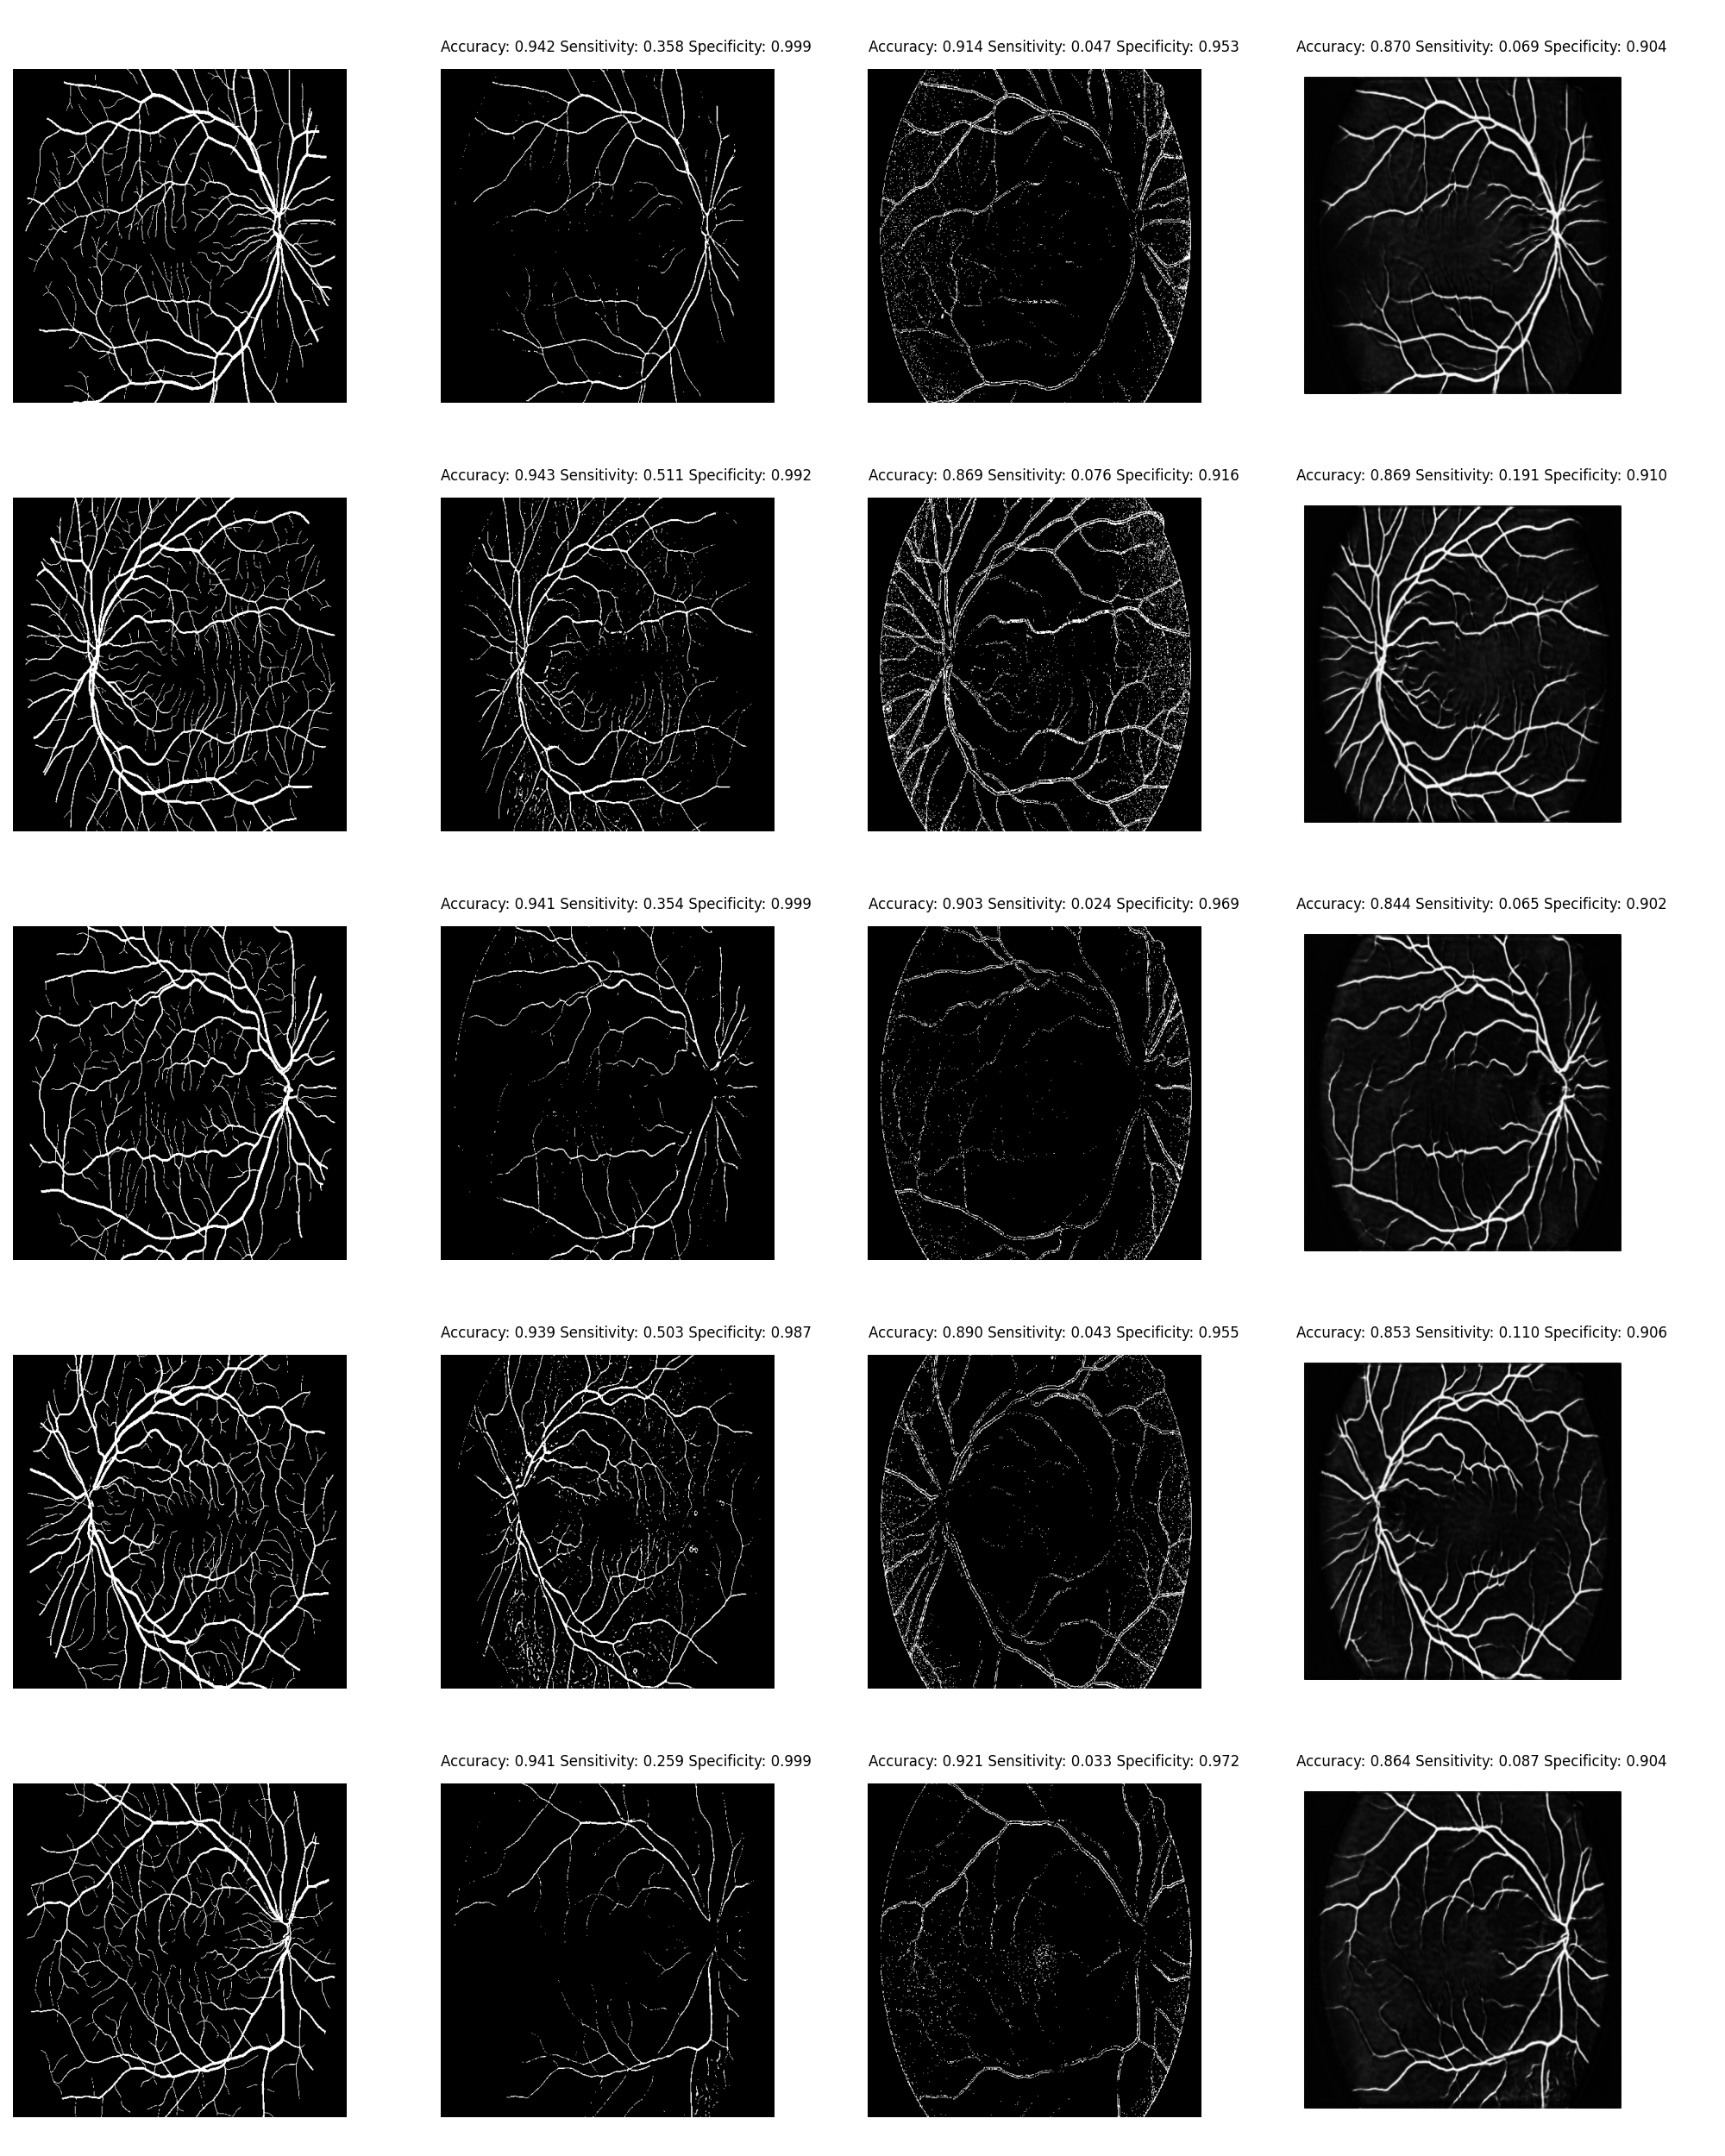
\includegraphics[width=\linewidth]{../res/predicted-images.png}
                                \end{minipage}
                            \end{figure}
                    \end{enumerate}
          \end{enumerate}
\end{enumerate}


\end{document}
